\section*{Câu 1 --- Perceptron cho đường biên}
Đường thẳng cho trước $x_2 = -\tfrac{3}{2}x_1 + 3$. Viết lại dạng $\mathbf{w}^\top\mathbf{x}+b=0$:
\[
\tfrac{3}{2}x_1 + x_2 - 3 = 0.
\]
Vậy có thể chọn $\mathbf{w} = \bigl(\tfrac{3}{2},\,1\bigr)^\top$, $b=-3$ (hoặc nhân hai vế cho số nguyên: $\mathbf{w}=(3,2)^\top$, $b=-6$).\\
Hàm kích hoạt $\tau(s)=+1$ nếu $s\ge 0$, $-1$ nếu $s<0$; đầu ra $y=\tau(\mathbf{w}^\top\mathbf{x}+b)$.

\section*{Câu 2}
\paragraph{(a)} Perceptron có trọng số bias $-3$, $x_1:2$, $x_2:1$ cho đường biên
\[
2x_1 + x_2 - 3 = 0.
\]

\paragraph{(b)} Với $\mathbf{x}^{(1)}=(-1,0)$: $s = 2(-1)+0-3=-5<0 \Rightarrow y=-1$.\\
Với $\mathbf{x}^{(2)}=(2,0)$: $s=4+0-3=1\ge 0 \Rightarrow y=+1$.

\paragraph{(c)} Đường qua $(2,0)$ và $(0,-1)$ có phương trình $x_1-2x_2-2=0$. Trong ký hiệu $w_0 + w_1x_1+w_2x_2=0$ trên biên, lấy $w_0=-2$, $w_1=1$, $w_2=-2$.

\paragraph{(d)} \textbf{OR:} các điểm $(1,0)$, $(0,1)$, $(1,1)$ mang nhãn $+1$, $(0,0)$ mang $-1$.\\
Chọn $s = -\tfrac{1}{2}+x_1+x_2$ (tức $w_0=-\tfrac{1}{2}$, $w_1=w_2=1$):\\
$(0,0)\Rightarrow s=-\tfrac{1}{2}$; $(1,0)$ và $(0,1)\Rightarrow s=\tfrac{1}{2}$; $(1,1)\Rightarrow s=\tfrac{3}{2}$ --- khớp bảng OR.\\
\textbf{AND:} chỉ $(1,1)$ mang $+1$. Với $s=-\tfrac{3}{2}+x_1+x_2$ ta có $(0,0),(1,0),(0,1)$ cho $s<0$ và $(1,1)$ cho $s=\tfrac{1}{2}\ge 0$.

\begin{figure}[htbp]
  \centering
  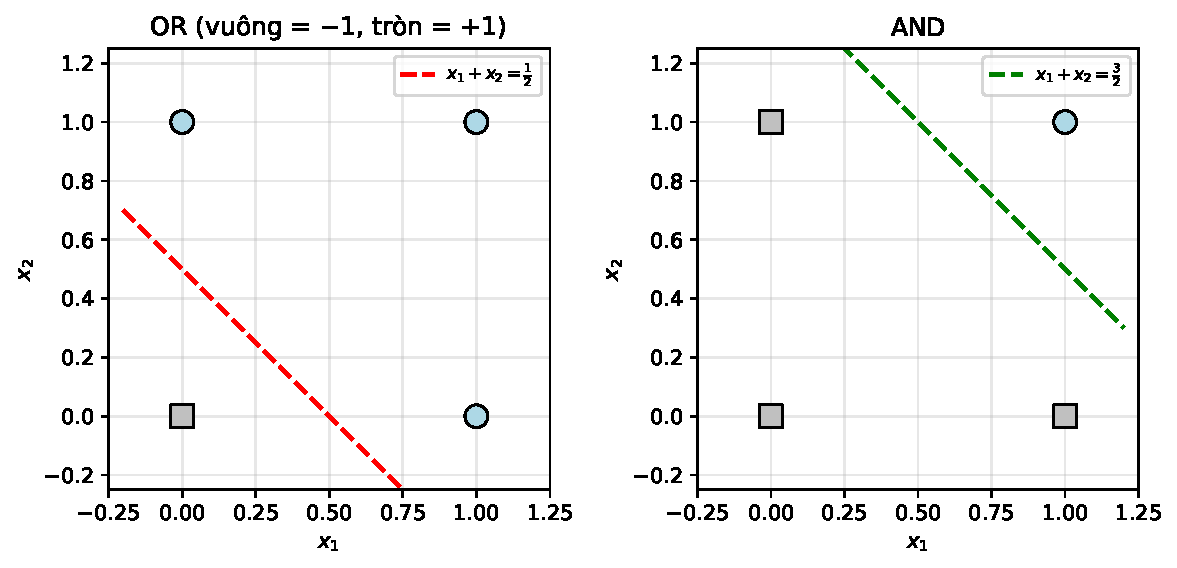
\includegraphics[width=0.92\linewidth]{figures/fig_or_and.pdf}
  \caption{Đường biên minh họa cho OR và AND (các trọng số đã chọn như trên).}
\end{figure}

\section*{Câu 3 --- Bảng OR}
Bốn mẫu $(x_1,x_2)$ với $(0,0)\mapsto -1$ và ba mẫu còn lại $\mapsto +1$ được phân đúng hoàn toàn bởi $s=-\tfrac{1}{2}+x_1+x_2$ như đã kiểm tra ở Câu~2(d).

\section*{Perceptron --- mất mát trên tập sai và GD batch}
\paragraph{(a)} Với $J(\mathbf{w},b)=\sum_{i\in Y}(-t_i)\bigl(\mathbf{w}^\top\mathbf{x}_i+b\bigr)$ ($Y$ là tập mẫu bị phân lớp sai),
\[
\frac{\partial J}{\partial \mathbf{w}}=\sum_{i\in Y}(-t_i)\mathbf{x}_i,\qquad
\frac{\partial J}{\partial b}=\sum_{i\in Y}(-t_i).
\]
Cập nhật gradient (bước $\rho>0$): $\mathbf{w}\leftarrow \mathbf{w}-\rho\,\partial J/\partial\mathbf{w}$, $b\leftarrow b-\rho\,\partial J/\partial b$.

\paragraph{(b)} \emph{Batch:} lặp cho đến khi không còn mẫu sai: mỗi vòng tìm tất cả chỉ số sai, gom vào $Y$; nếu $Y=\varnothing$ thì dừng; nếu không, cập nhật một lần từ toàn bộ $Y$ như trên.

\paragraph{(c)} Đường ngang $x_2=\tfrac{1}{2}$ tương đương $0\cdot x_1 + 1\cdot x_2 - \tfrac{1}{2}=0$, nên khởi tạo $\mathbf{w}(0)=(0,1)^\top$, $b(0)=-\tfrac{1}{2}$.

\paragraph{(d)} Với $\rho=\tfrac{2}{5}$, bước khởi tạo chỉ sai mẫu $(1,0)$ nhãn $+1$. Ta có $\partial J/\partial\mathbf{w}=(-1,0)^\top$, $\partial J/\partial b=-1$, nên sau một bước $\mathbf{w}=\bigl(\tfrac{2}{5},1\bigr)^\top$, $b=-\tfrac{1}{10}$ và mọi mẫu đều đúng. Các đường biên ở từng bước được vẽ trong hình sau.

\begin{figure}[htbp]
  \centering
  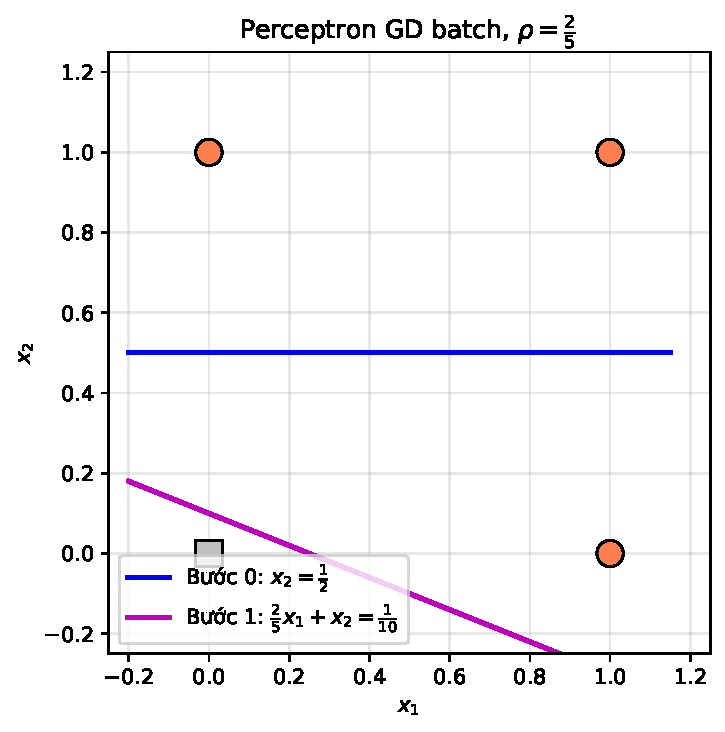
\includegraphics[width=0.62\linewidth]{figures/fig_perceptron_gd.pdf}
  \caption{Các đường phân cách trước và sau một bước GD batch ($\rho=0{,}4$).}
\end{figure}

\section*{Câu 4 --- Lan truyền thuận MLP}
Đầu vào $(x_1,x_2)=(1,1)$, hàm $\tau$ là dấu.\\
Neuron~1: $s_1=-\tfrac{1}{2}+1+1=\tfrac{3}{2}\ge 0 \Rightarrow +1$.\\
Neuron~2: $s_2=\tfrac{3}{2}-1-1=-\tfrac{1}{2}<0 \Rightarrow -1$.\\
Neuron~3: $s_3=-1+(+1)+(-1)=-1<0 \Rightarrow -1$.

\section*{Câu 5 --- Hồi quy tuyến tính một chiều}
Bốn điểm $(0,1)$, $(1,3)$, $(2,5)$, $(3,7)$ nằm trên đường thật $y=2x+1$. Đặt $m=4$, $J(w,b)=\dfrac{1}{2m}\sum_{i=1}^4\bigl(y_i-wx_i-b\bigr)^2$.

\paragraph{(a)} Đạo hàm
\[
\frac{\partial J}{\partial w}=-\frac{1}{m}\sum_{i=1}^m\bigl(y_i-wx_i-b\bigr)x_i,\qquad
\frac{\partial J}{\partial b}=-\frac{1}{m}\sum_{i=1}^m\bigl(y_i-wx_i-b\bigr).
\]
Cập nhật: $w\leftarrow w-\rho\,\partial J/\partial w$, $b\leftarrow b-\rho\,\partial J/\partial b$.

\paragraph{(b)} Tại điểm khởi tạo của mục~(c) dưới đây ($w=0$, $b=1$, tức $\hat y\equiv 1$), phần dư $(y_i-\hat y_i)$ lần lượt là $0,2,4,6$; suy ra
\[
\frac{\partial J}{\partial w}=-\tfrac{1}{4}(0+2+8+18)=-7,\qquad
\frac{\partial J}{\partial b}=-\tfrac{1}{4}(0+2+4+6)=-3,
\]
và $J=\dfrac{1}{8}(0^2+2^2+4^2+6^2)=\dfrac{56}{8}=7$.

\paragraph{(c)} Đường nằm ngang $\hat y=1$ ứng $w(0)=0$, $b(0)=1$.

\paragraph{(d)} Với $\rho=0{,}1$, ba vòng lặp cho
\begin{center}
\begin{tabular}{@{}rlll@{}}
Vòng & $w$ & $b$ & $J$ \\ \hline
$0$ & $0$ & $1$ & $7$ \\
$1$ & $0{,}7$ & $1{,}3$ & $2{,}4175$ \\
$2$ & $1{,}11$ & $1{,}465$ & $0{,}8735125$ \\
$3$ & $1{,}35175$ & $1{,}552$ & $\approx 0{,}3510$
\end{tabular}
\end{center}
(chữ số thêm của $J$ sau vòng $3$ là $0{,}351000109375$, không ảnh hưởng mục đích minh họa).

\paragraph{(e)} Hình~\ref{fig:reg} minh học các đường hồi quy sau từng vòng.

\begin{figure}[htbp]
  \centering
  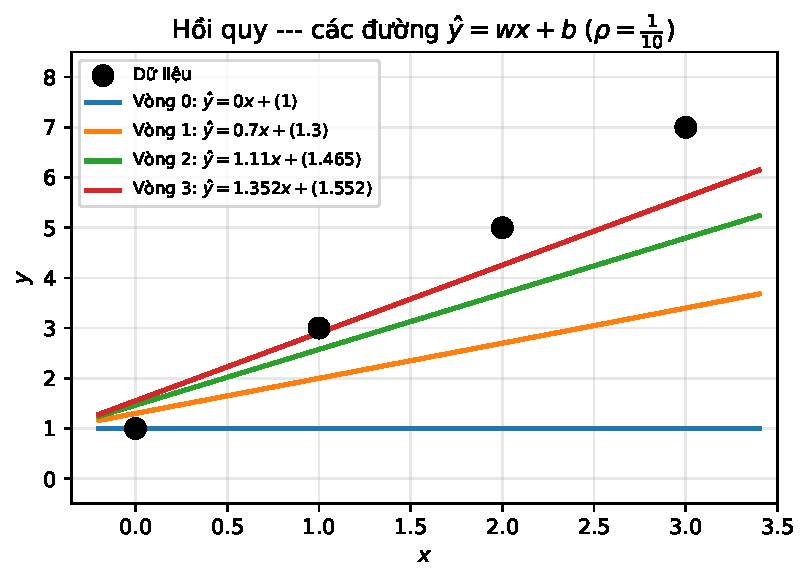
\includegraphics[width=0.7\linewidth]{figures/fig_regression_gd.pdf}
  \caption{Các đường $\hat y=wx+b$ qua các vòng GD ($\rho=0{,}1$).}
  \label{fig:reg}
\end{figure}

\section*{Phần học sâu --- kích thước CNN và tích chập tay}
\paragraph{(a)} Đầu vào $128\times 128\times 3$, cửa sổ $3\times 3$, stride $2$, padding $1$:
\[
H_{\text{out}}=\left\lfloor\frac{128+2-3}{2}\right\rfloor+1=64
\]
(và tương tự chiều rộng). Độ sâu bằng số filter: $a=32$, nên tensor ra $64\times 64\times 32$ (chiều cao $c=64$, chiều rộng $b=64$ theo ký hiệu hình vẽ).

\paragraph{(b)} Đặt
\[
X=\begin{bmatrix}4&6&3&4\\1&7&3&4\\5&8&4&4\\2&7&4&4\end{bmatrix},\quad
K=\begin{bmatrix}0&-\tfrac14&0\\-\tfrac14&1&-\tfrac14\\0&-\tfrac14&0\end{bmatrix}.
\]
Tích chập \emph{valid} cho ma trận $2\times 2$:
\[
\begin{bmatrix} 2{,}5 & -1{,}5 \\ 2{,}25 & -0{,}75 \end{bmatrix}.
\]
Max-pooling $2\times 2$ (một ô) lấy $\max\{2{,}5,-1{,}5,2{,}25,-0{,}75\}=2{,}5$.

\section*{Câu 6 --- MLP nhận dạng chữ số}
Ảnh $10\times 10$ vectơ hoá thành $n\in\mathbb{R}^{100}$. Lớp ẩn $k$ nút: $m=W^{(1)}n+b^{(1)}$, $h=\mathrm{ReLU}(m)$, $z=W^{(2)}h+b^{(2)}$, $y=\mathrm{softmax}(z)$ (đề ghi nhầm $\mathrm{softmax}(x)$, đúng ra biến đổi vào tầng tuyến tính cuối).\\
\textbf{(a)} $\dim y=10$ (mười lớp chữ số).\\
\textbf{(b)} $W^{(1)}\in\mathbb{R}^{k\times 100}$, $W^{(2)}\in\mathbb{R}^{10\times k}$ (hoặc chuyển vị tùy quy ước cột/ hàng, nhưng cặp kích thước là $(k,100)$ và $(10,k)$).

\section*{Câu 7 --- CNN theo mô tả Keras}
Luồng kích thước: $28\times28\times1 \rightarrow 26\times26\times64 \rightarrow 26\times26\times64 \rightarrow 13\times13\times64 \rightarrow 10816 \rightarrow 128 \rightarrow 10$.\\
Tham số:
\begin{itemize}\itemsep0.25em
\item Conv2D $(3\cdot 3\cdot 1+1)\cdot 64 = 640$.
\item Dense-1 $10816\cdot 128 + 128 = 1\,384\,576$.
\item Dense-2 $128\cdot 10 + 10 = 1290$.
\end{itemize}
Bảng tóm tắt (độ lớn đầu ra --- lớp phi tuyến không thêm tham số):

\begin{center}
\small
\begin{tabular}{@{}lcc@{}}
Lớp & Kích thước tensor & Tham số \\ \hline
Input & $28\times 28\times 1$ & $0$ \\
Conv2D+ReLU & $26\times 26\times 64$ & $640$ \\
MaxPool & $13\times 13\times 64$ & $0$ \\
Flatten & $10816$ & $0$ \\
Dense-1+ReLU & $128$ & $1\,384\,576$ \\
Dense-2+softmax & $10$ & $1290$ \\
\end{tabular}
\end{center}

\begin{figure}[htbp]
  \centering
  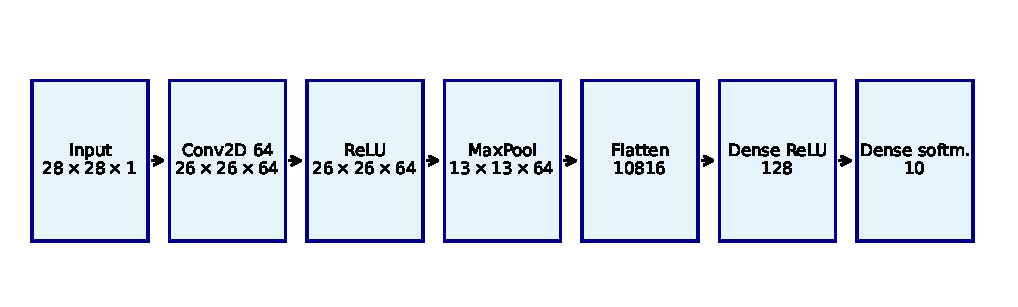
\includegraphics[width=\linewidth]{figures/fig_cnn_arch.pdf}
  \caption{Sơ đồ khối và kích thước các tầng CNN (Câu~7).}
\end{figure}

\section*{Câu 8 --- RNN}
Với ma trận $U,W,V$ và bias phù hợp kích thước, dùng $\tanh$ cho trạng thái và $\mathrm{softmax}$ cho đầu ra:
\[
s_t=\tanh(Ux_t + W s_{t-1} + b),\qquad
o_t=\mathrm{softmax}(V s_t + c).
\]

\section*{Câu 9 --- Công thức LSTM}
Ký hiệu nối vector $[h_{t-1},x_t]$, $\sigma$ là sigmoid, $\odot$ là nhân từng phần tử:
\begin{align*}
f_t &= \sigma\bigl(W_f[h_{t-1},x_t]+b_f\bigr), &
i_t &= \sigma\bigl(W_i[h_{t-1},x_t]+b_i\bigr),\\
\tilde C_t &= \tanh\bigl(W_C[h_{t-1},x_t]+b_C\bigr), &
C_t &= f_t\odot C_{t-1} + i_t\odot \tilde C_t,\\
o_t &= \sigma\bigl(W_o[h_{t-1},x_t]+b_o\bigr), &
h_t &= o_t\odot \tanh(C_t).
\end{align*}
